\documentclass[8pt]{beamer}

\usepackage{listings}

\definecolor{codegreen}{rgb}{0,0.6,0}
\definecolor{codegray}{rgb}{0.5,0.5,0.5}
\definecolor{codepurple}{rgb}{0.58,0,0.82}
\definecolor{backcolour}{rgb}{0.95,0.95,0.92}

\lstdefinestyle{mystyle}{
backgroundcolor=\color{backcolour},
commentstyle=\color{codegreen},
keywordstyle=\color{magenta},
numberstyle=\tiny\color{codegray},
stringstyle=\color{codepurple},
basicstyle=\ttfamily\small,
breakatwhitespace=false,
breaklines=true,
captionpos=b,
keepspaces=true,
numbers=left,
numbersep=5pt,
showspaces=false,
showstringspaces=false,
showtabs=false,
tabsize=2
}

\usetheme[sectionpage=none]{metropolis}
\setbeamertemplate{section in toc}[sections numbered]

\title{Developing the OpenTURNS documentation}
\author{Joseph MUR\'E - EDF R\&D}
\date{February 14th-17th 2022}
\titlegraphic{\includegraphics[height=1.5cm]{logoOT}}
\institute{\small OpenTURNS Consortium}


\begin{document}

\frame{\titlepage}

% necessaire pour la table des matieres
\part{Main part}

%%%%%%%%%%%%%%%%%%%%%%%%%%%%%%%%%%
% The development infrastructure %
%%%%%%%%%%%%%%%%%%%%%%%%%%%%%%%%%%

\begin{frame}
  \frametitle{A few words about the development infrastructure (1/2)}
  \begin{block}{Versioning system}
    \begin{itemize}
    \item \alert{Git} is a software versioning and a revision control system started by Linus Torvalds. It is used for the sources of the platform, the documentation, as well as for the development of modules.
    \item \alert{GitHub} is a web-based hosting service for version control using Git.
    GitHub provides a bug tracker, pull requests (GitLab equivalent: merge requests), continuous integration, and other features.
    \end{itemize}
  \end{block}
  \begin{block}{Official repository and forks}
    The \alert{official repository} of the library is \url{https://github.com/openturns/openturns}.
    \begin{itemize}
    \item All developers have a \alert{fork} of that repository to host their development branches.
    \item Only the \alert{integrator} (and a backup) has write access to the official repository.
    \item Modules are not part of the library, but some of them are maintained by the consortium: their repositories are hosted at \url{https://github.com/openturns}
    and they have the same development process as the library.
    \item Other modules are hosted elsewhere and do not need to follow the same development process.
    \end{itemize}
  \end{block}
\end{frame}

\begin{frame}
    \frametitle{A few words about the development infrastructure (2/2)}
    \begin{block}{Structure of the library repository}
    The repository of the library contains source code for the C++ library, the Python interface and the documentation. Its layout is quite standard:
    \begin{itemize}
    \item A \alert{master branch} that stores the source code of the upcoming version of the platform. The rule is to have only source code that passes all tests.
    \item Branches for \alert{stable versions} and \alert{tags for releases} and release candidates.
    \item Development branches are part of \alert{contributor forks}.
    \item Development branches are merged with master via \alert{pull requests}.
    \item At least \alert{2 reviewers must approve} the PR, and unanimity is required.
    \end{itemize}
  \end{block}

  \begin{block}{Continuous integration}
    OpenTURNS makes extensive use of online continuous integration providers to \alert{test the library} throughout the development process. Currently the following services are used to test the library:
    \begin{itemize}
    \item CircleCI: Linux and MinGW
    \item GitHub Actions: macOS and Windows
    \end{itemize}
  \end{block}
\end{frame}

\begin{frame}{OpenTURNS development workflow}
    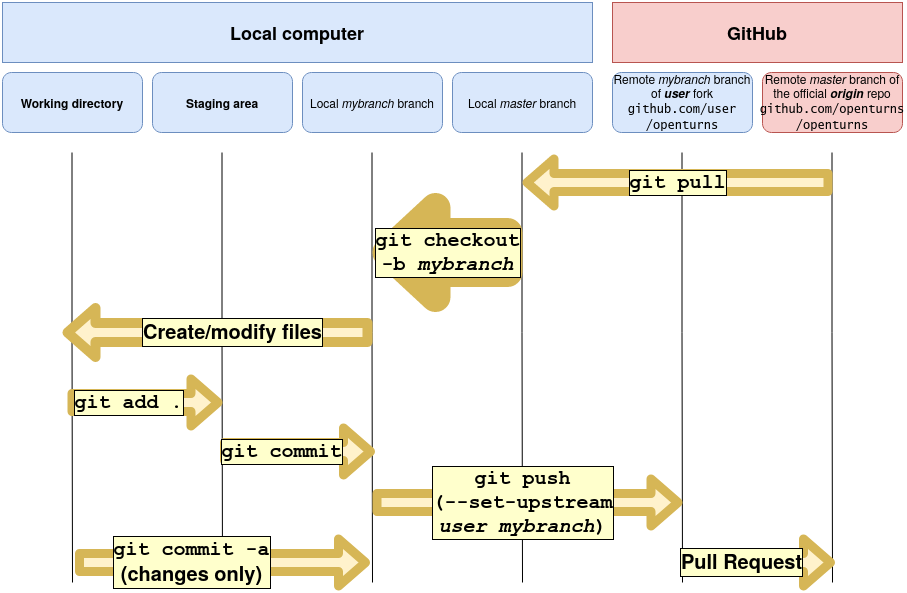
\includegraphics[width=\textwidth]{Git_flow.png}
\end{frame}

%%%%%%%%%%%%%%%%%%%%%
% All doc sections  %
%%%%%%%%%%%%%%%%%%%%%

\begin{frame}{Overview of the OpenTURNS documentation}
The OpenTURNS documentation is built using the Python \href{https://www.sphinx-doc.org/en/master/index.html}{\alert{Sphinx}} package.

One of the Continuous Integration machines (CircleCI \texttt{build-linux})
produces the documentation and publishes it online.
Several versions are online:

\begin{itemize}
\item The version corresponding to the current release has \alert{\texttt{latest}} in its URL:
\url{https://openturns.github.io/openturns/latest/}
\item The version corresponding to the master branch has \alert{\texttt{master}} in its URL:
\url{https://openturns.github.io/openturns/master/}
\item Older versions are accessible with the version number: \url{https://openturns.github.io/openturns/1.17/}
\end{itemize}

If you spot a mistake, make sure you are looking at \texttt{master} before correcting!

The built-in search engine distinguishes between 3 main sections:

\begin{itemize}
    \item \alert{Examples}
    \item \alert{API} (user manual)
    \item \alert{Theory}
\end{itemize}

You may also want to check out:

\begin{itemize}
    \item \alert{Contribute} (developer guide)
    \item \alert{Common use cases} (added in 2020)
\end{itemize}
\end{frame}

%%%%%%%%%%%%%%%%%%%%%
% Theory            %
%%%%%%%%%%%%%%%%%%%%%
\section{Theory}

% Outline
\begin{frame}[label=tableofcontents]
\frametitle{Outline}
\tableofcontents[currentsection]
\end{frame}


\begin{frame}{Looking up the source file of a theory page}


Let us consider the \alert{Using QQ-plot to compare two samples} page:

\url{https://openturns.github.io/openturns/master/theory/data_analysis/qqplot_graph.html}

All Theory files are RST and the URL fits the source folder structure, so the relevant source file is:
\href{https://github.com/openturns/openturns/blob/master/python/doc/theory/data_analysis/qqplot_graph.rst}{\texttt{python/doc/theory/data\_analysis/qqplot\_graph.rst}}

There are great RST and Sphinx \href{https://thomas-cokelaer.info/tutorials/sphinx/rest_syntax.html}{\alert{cheatsheet}} available,
but here are the basics:

\begin{itemize}
    \item A page can be \alert{indexed} as \texttt{page\_name} by writing \texttt{.. \_page\_name:} at the top.
    \item Because of this, that page can be \alert{linked} to from anywhere in the doc with \texttt{:ref:`page\_name`}
    \item \alert{Titles} are underlined (the number of underlining characters must match the title).
    \item \alert{Inline math} is \LaTeX{} code with \texttt{\$a=b\$} replaced with \texttt{:math:`a=b`}.
    \item \alert{Display math} is \LaTeX{} code with \texttt{\$\$a=b\$\$} replaced with
    
    \texttt{.. math::}
    
    \texttt{~~~~a = b}
    \item \alert{Macros} are defined in \href{https://github.com/openturns/openturns/blob/master/python/doc/math_notations.sty}{\texttt{python/doc/math\_notations.sty}}
    \item Try to use notations \alert{consistent} with other theory pages.
    \item The \alert{bibliography} can be found at \href{https://github.com/openturns/openturns/blob/master/python/doc/bibliography.rst}{\texttt{python/doc/bibliography.rst}}
\end{itemize}

\end{frame}


\begin{frame}[fragile]{Adding a new theory page}
Code of the main table of contents (\href{https://github.com/openturns/openturns/blob/master/python/doc/theory/theory.rst}{python/doc/theory/theory.rst}):

\lstset{style=mystyle}

\begin{lstlisting}
.. _theory:

======
Theory
======

The theoretical documentation.
This contains an in-depth description of all algorithms.

.. toctree::
    :maxdepth: 2

    data_analysis/data_analysis.rst
    probabilistic_modeling/probabilistic_modeling.rst
    meta_modeling/meta_modeling.rst
    reliability_sensitivity/reliability_sensitivity.rst
    numerical_methods/numerical_methods.rst
\end{lstlisting}
Table of contents of subdirectories are essentially the same.

What holds for the \alert{Theory} section also mostly holds for the \alert{Contribute} (developer guide) and \alert{Common use cases} sections.
\end{frame}



%%%%%%%%%%%%%%%%%%%%%
% Examples          %
%%%%%%%%%%%%%%%%%%%%%
\section{Examples}

\againframe<2>{tableofcontents}


\begin{frame}{Looking up the source Python script of an example}

The Examples section is produced by \href{https://sphinx-gallery.github.io/stable/index.html}{\alert{Sphinx-gallery}}, a Sphinx extension.

Let us consider the \alert{Kriging with an isotropic covariance function} example:

\url{https://openturns.github.io/openturns/master/auto_meta_modeling/kriging_metamodel/plot_kriging_isotropic.html}

Example source files are \alert{Python scripts}.
The URL is still linked to the the source folder structure,
but the \texttt{auto\_} part is a Sphinx-gallery artifact. Its source file is:

\href{https://github.com/openturns/openturns/blob/master/python/doc/examples/meta_modeling/kriging_metamodel/plot_kriging_isotropic.py}{\texttt{python/doc/examples/meta\_modeling/kriging\_metamodel/\\plot\_kriging\_isotropic.py}}

\begin{itemize}
    \item Use \alert{\texttt{\# \%\%}} to start a \alert{new cell}.
    \item Write \alert{Python code} as you \alert{normally} would.
    \item Write \alert{text as RST code}, but each RST line must start with \alert{\texttt{\#}}.
    \item A cell can contain both RST and Python code, but \alert{RST must come first}.  
    \item \alert{RST rules are the same} as in the Theory section.
    \item A \alert{blank line} interrupts RST code and \alert{switches to Python}. For the remainder of the cell, lines starting with \alert{\texttt{\#}} are simply interpreted as Python comments.
    \item By default, the first image is used as \alert{thumbnail picture}. To use e.g. the third: %$n$\textsuperscript{rd} image:%, write (preferably right above the code that produces the image):

    \texttt{\# sphinx\_gallery\_thumbnail\_number = 3} (ideally right above the plot code)
    \item In the \alert{script docstring}, \LaTeX{} backslashes \texttt{\textbackslash} need to be doubled: \texttt{\textbackslash\textbackslash}
\end{itemize}

\end{frame}


\begin{frame}{Adding a new example}
\begin{itemize}
    \item Normally, you should not need to change \href{https://github.com/openturns/openturns/blob/master/python/doc/examples/examples.rst}{\texttt{python/doc/examples/examples.rst}}.
    \item Every subfolder has a \alert{\texttt{README.txt}} file, which is actually an RST file that only contains a label for hypertext links and the subsection title.
    \item All source Python scripts are \alert{automatically detected} and used to build HTML examples and the corresponding thumbnails, provided their name follows the \texttt{plot\_xxx.py} template.
    \item \alert{No need to index the files}, just put them in the appropriate subfolder.
    \item You can use the \alert{docstring} at the start of the file not only to write the title of the example, but also the introductory text. This docstring is the only part of the script that is interpreted as RST code without a \alert{\texttt{\#}} at the start of every line.
    \item \alert{Hypertext links} help users connect various aspects of the library:
    \begin{itemize}
        \item \texttt{:class:`\textasciitilde openturns.ClassName`} to link to the API doc of a class.
        \item \texttt{:meth:`\textasciitilde openturns.ClassName.method`} to link to the API doc of a class method.
        \item \texttt{:ref:`\_theory\_page`} to link to a Theory doc page using its RST label.
        \item \texttt{:doc:`/auto\_category/subcategory/plot\_xxx`} (no \texttt{.py}) to link to another example.
    \end{itemize}
    \item Python scripts should be properly
    formatted according to the \href{https://www.python.org/dev/peps/pep-0008/}{\alert{PEP8}}.

    Use \href{https://github.com/psf/black}{\alert{Black}} to format them automatically if needed.
    \item  Examples should \alert{combine several classes} in order to \alert{do something useful}.
\end{itemize}
\end{frame}

\begin{frame}[fragile]{Examples section: write interesting English (1/2)}
In the Examples section, the English content should be an interesting explanation
of the Python content. \medskip

\textbf{Do not write:}


\lstset{style=mystyle, language=python}

\begin{lstlisting}
# %%
# Draw the function

n = 10000
sampleX = im.distributionX.getSample(n)
sampleY = im.model(sampleX)
[...]
plotXvsY(sampleX, sampleY)
\end{lstlisting}

\end{frame}


\begin{frame}[fragile]{Examples section: write interesting English (2/2)}
\lstset{style=mystyle, language=python}

\textbf{Write instead:}

\begin{lstlisting}
# %%
# In the next cell, we create a large sample of the input random
# vector and evaluate the corresponding output from the physical
# model. We then create a function which takes the input and output
# samples as input argument and creates a grid of scatter plots.

n = 10000
sampleX = im.distributionX.getSample(n)
sampleY = im.model(sampleX)
[...]
plotXvsY(sampleX, sampleY)

# %%
# We see that the variance of the output is mostly sensitive to the
# first variable :math:`X_1`.
# The variance of the output is not sensitive to the third
# variable, since the conditional variance is zero.
\end{lstlisting}
\end{frame}

%%%%%%%%%%%%%%%%%%%%%
% API (user manual) %
%%%%%%%%%%%%%%%%%%%%%
\section{API (user manual)}

\againframe<3>{tableofcontents}


\begin{frame}
\frametitle{SWIG: Simplified Wrapper and Interface Generator}
\begin{block}{A tool to link C/C++ libraries with script languages}
    SWIG parses the library headers (\texttt{.hxx}) and swig interface files (\texttt{.i}) to
    generate the corresponding module source that must be compiled to
    produce a binary Python module.
\end{block}
\centering \resizebox{!}{4cm}{\includegraphics{swig.png}} \medskip

Python \alert{docstrings} are written in \texttt{\_doc.i.in} files which supplement the \alert{SWIG} \texttt{.i} files.

These docstrings are then read by \alert{Sphinx} to build the API doc section.
\end{frame}


\begin{frame}{Looking up the sources of docstrings}
Let us consider the \alert{LinearCombinationFunction} class and its source file:
\url{https://openturns.github.io/openturns/master/user_manual/_generated/openturns.LinearCombinationFunction.html}
\href{https://github.com/openturns/openturns/blob/master/python/src/LinearCombinationFunction_doc.i.in}{python/\alert{src}/LinearCombinationFunction\_doc.i.in}

\begin{itemize}
    \item Docstring sources are in \texttt{src} rather than \texttt{doc} because they are \alert{part of the library}.
    \item A docstring is \alert{just a string} \texttt{"..."}: double quotes are thus forbidden inside, use \texttt{'...'} instead (not to be confused with \texttt{`...`} as in \texttt{:math:`...`}). Do not put any whitespace between the opening \texttt{"} and the first docstring character, nor between the last docstring character and the closing \texttt{"}.
    \item Docstrings follow \href{https://numpydoc.readthedocs.io/en/latest/index.html}{\alert{Numpydoc}} style. \alert{RST rules remain the same.}
    \item Example code lines start with \alert{\texttt{>{}>{}>}} and are run during Python tests! If you call \texttt{print}, you need to \alert{specify the expected output} or the test will fail.
    \item Numerical values can differ slightly between platforms.
    To prevent CI failures, you may replace the last digits with an \alert{ellipsis}: \texttt{0.34023...} instead of \texttt{0.3402362897}
    \item Class inheritance extends to docstrings: \texttt{LinearCombinationFunction} inherits all its method docstrings from \alert{\texttt{FunctionImplementation}}: look for the docstrings in \href{https://github.com/openturns/openturns/blob/master/python/src/FunctionImplementation_doc.i.in}{\texttt{python/src/FunctionImplementation\_doc.i.in}}.
    \item \texttt{FunctionImplementation} has no HTML page, although it has many docstrings.
    Instead, those docstrings are used to produce the \href{https://openturns.github.io/openturns/master/user_manual/_generated/openturns.Function.html}{\alert{HTML file}}
    of \href{https://github.com/openturns/openturns/blob/master/python/src/Function_doc.i.in}{\alert{Function}}.
    This holds for almost all Interface/Implementation couples.
\end{itemize}
    
\end{frame}


\begin{frame}{Docstrings of a new class and/or method: SWIG part}
To get the \alert{docstrings} to appear \alert{in the Python library}, you need to act on \alert{\texttt{python/src}}:
\begin{itemize}
    \item Create a \alert{docstring file} \texttt{MyClass\_doc.i.in}
    \item Declare the \alert{class docstring}: \texttt{\%feature("docstring") OT::MyClass}
    \item Declare a \alert{method docstring}: \texttt{\%feature("docstring") OT::MyClass::myMethod}
    \item Two ways are available to actually create the docstring:
    \begin{enumerate}
        \item Write the docstring between double-quotes \alert{right under the declaration}.
        \item \alert{Make it a variable} so it can be used in several different places:

        \texttt{\%define OT\_MyClass\_(myMethod)\_doc}

        \texttt{"..."}

        \texttt{\%enddef}
    \end{enumerate}
    \item For a new class, \alert{do not forget to declare}:
    \begin{itemize}
        \item the docstrings in \alert{\texttt{MyClass.i}}: \texttt{\%include MyClass\_doc.i}
        \item the class in the appropriate \alert{\texttt{xxx\_module.i}}: \texttt{\%include MyClass.i}
        \item the class and its docstrings in the appropriate \texttt{xxx\_module} section of \alert{\texttt{CMakeLists.txt}}: \texttt{MyClass.i MyClass\_doc.i.in}
    \end{itemize}    
    \item For a new Interface/Implementation couple, define the docstrings in \texttt{XxxImplementation\_doc.i.in} with \alert{\texttt{\%define}} to be able to reuse them in the Interface docstrings file \texttt{Xxx\_doc.i.in}: see \href{https://github.com/openturns/openturns/blob/master/python/src/Function_doc.i.in}{\texttt{Function\_doc.i.in}} and \href{https://github.com/openturns/openturns/blob/master/python/src/FunctionImplementation_doc.i.in}{\texttt{FunctionImplementation\_doc.i.in}} for example.
\end{itemize}
\end{frame}


\begin{frame}{Docstrings of a new class: Sphinx part}
Sphinx looks at \href{https://github.com/openturns/openturns/tree/master/python/doc/user_manual}{\texttt{python/\alert{doc}/user\_manual}} for the structure of the API documentation.

For example, \href{https://openturns.github.io/openturns/master/user_manual/_generated/openturns.LinearCombinationFunction.html}{\alert{LinearCombinationFunction}} is referenced in \href{https://github.com/openturns/openturns/blob/master/python/doc/user_manual/functions.rst}{\texttt{python/doc/user\_manual/functions.rst}}

To get your new class to appear in the \alert{HTML API doc} section:

\begin{itemize}
    \item Find the \alert{RST file} of the appropriate subsection.
    \item \alert{Insert the name} of your class where you want it to appear.
    \item Make sure it uses the correct \alert{template}, otherwise use the \texttt{:template:} directive.
\end{itemize}

Templates are found in the \href{https://github.com/openturns/openturns/tree/master/python/doc/_templates}{\texttt{python/doc/\_templates}} folder. The main templates are:

\begin{itemize}
    \item \href{https://github.com/openturns/openturns/blob/master/python/doc/_templates/class.rst_t}{\alert{\texttt{class.rst\_t}}}
    \item \href{https://github.com/openturns/openturns/blob/master/python/doc/_templates/classWithPlot.rst_t}{\alert{\texttt{classWithPlot.rst\_t}}}
\end{itemize}

If you want to use \texttt{classWithPlot.rst\_t}, you need to provide the code to generate the graph at the top of the page. For example, \href{https://openturns.github.io/openturns/master/user_manual/_generated/openturns.LinearCombinationFunction.html}{\alert{LinearCombinationFunction}} runs the code in
\href{https://github.com/openturns/openturns/blob/master/python/doc/pyplots/LinearCombinationFunction.py}{\texttt{\alert{python/doc/pyplots}/LinearCombinationFunction.py}}.

Note that the plot code can be downloaded from the API doc page itself by clicking on ``\emph{Source code}''.
\end{frame}

\begin{frame}[fragile]{API example: always document the most significant method}

\lstset{style=mystyle, language=python}

In the API documentation, the \alert{most significant method} should have an
example within the main section, at the top of the help page.
This main example should document the \alert{\emph{flagship}} of the class, that is, 
the most significant method(s) of the class.

For example, one of the main features of the \href{https://openturns.github.io/openturns/master/user_manual/_generated/openturns.LinearEnumerateFunction.html}{\alert{LinearEnumerateFunction}}
class is its evaluation operator, which is why the first example is:

\begin{lstlisting}
>>> import openturns as ot
>>> enumerateFunction = ot.LinearEnumerateFunction(2, 0.5)
>>> for i in range(10):
>>>     print(enumerateFunction(i))
\end{lstlisting}

Constrast with examples from the \alert{Examples} section,
which \alert{combine several classes} in order to do useful Uncertainty Quantification.
\end{frame}


\begin{frame}{Summary of the previous parts}
Two tools are involved in the creation of the documentation.

\textbf{Sphinx}:
\begin{itemize}
    \item Theory files: \texttt{python/\alert{doc}/theory}
    \item Example files: \texttt{python/\alert{doc}/examples}
    \item API tables of contents: \texttt{python/\alert{doc}/user\_manual}
    \item API plots: \texttt{python/\alert{doc}/pyplots}
    \item Math notations are defined in \href{https://github.com/openturns/openturns/blob/master/python/doc/math_notations.sty}{\texttt{python/\alert{doc}/math\_notations.sty}}
\end{itemize}

\textbf{SWIG}:
\begin{itemize}
    \item API docstrings: \texttt{*\_doc.i.in} files in \texttt{python/\alert{src}}
\end{itemize}

Docstrings are in \texttt{python/\alert{src}} because they are part of the Python library and not only the HTML documentation.

\end{frame}



%%%%%%%%%%%%%%%%%%%%%
% Tips and tricks   %
%%%%%%%%%%%%%%%%%%%%%
\section{Tips and tricks}

\againframe<4>{tableofcontents}


\begin{frame}{Quickly find the appropriate source file}

The GitHub \href{https://github.com/openturns/openturns/find/master}{``\alert{\emph{Go to file}}''} button does wonders to find the source file you need.

\includegraphics[width=\textwidth]{Github_gotofile}

\begin{itemize}
    \item API: simply type the class name.
    \item Examples: scroll down to ``\alert{\emph{Download Python source code}}'' for the script name.
    \item Theory: click on ``\alert{\emph{Show source}}'', the exact \texttt{.rst} file name appears in the URL.
\end{itemize}

\end{frame}


\begin{frame}[fragile]{Write clear commit messages: examples}

\lstset{style=mystyle}

\begin{lstlisting}
Create a quick start example for points and samples
\end{lstlisting}

\begin{lstlisting}
Add new ResourceMap keys for Mesh checking

We add a new RM key for mesh checking. Default value is set to False
as the method might be costly.
\end{lstlisting}

\begin{lstlisting}
Doc: Fix keyword in graph example

Closes #1742
\end{lstlisting}

\begin{lstlisting}
Fixed GaussianNonLinearCalibration

The estimation of distribution of the observations error was
incorrect. It was created using a zero mean to compute the Cholesky
factor of its (known) covariance matrix in order to compute the
residual function, but was not updated once the residual function
was known.

Closes #1529
\end{lstlisting}

\end{frame}

\begin{frame}{Write clear commit messages: the rules}
    \begin{itemize}
        \item First line: a \alert{title} of 50 characters or less.
        \item Second line: \alert{blank}
        \item Next lines: \alert{body} of the message with unlimited length.
        \item If your commit \alert{closes an issue}, use one of the following keywords in the body:
        \begin{itemize}
            \item \texttt{Close \#....}
            \item \texttt{Closes \#....}
            \item \texttt{Fix \#....}
            \item \texttt{Fixes \#....}
            \item \texttt{Solve \#....}
            \item \texttt{Solves \#....}
        \end{itemize}
    \end{itemize}

    Some text editors like Vim use syntax coloring to help you remember these rules.

    Closing keywords are recognized by GitHub: when your commit enters the master branch,
    the corresponding issue is \alert{automatically closed}.

    Remember to also use these \alert{keywords in the first message} of your \alert{pull request},
    so that GitHub registers the PR as fixing the issue.

    The first message of the PR should \alert{summarize the changes} made by the commits of the PR.


\end{frame}

\begin{frame}{Tip for reviewers: always look at the HTML output, not the source file!}
CircleCI \texttt{build\_linux} builds the doc in addition to the library when a PR is submitted.

For easy access, click on the ``\alert{\emph{Details}}'' link of the \texttt{build\_linux artifact} ``check''.

\includegraphics[width=0.9\textwidth]{Github_checks}

\begin{itemize}
    \item The \texttt{build\_linux artifact} pseudo-check ``succeeds'' if, and only if, the \texttt{build\_linux} check succeds.
    This means that a test failure could cause a red cross to appear in front of both of them, even though the doc was actually successfully generated.
    \item If the person submitting the Pull Request has CircleCI set up on their fork, then the \texttt{build\_linux artifact} link is always broken regardless of whether or not the doc was successfully built. You can still access it through the ``\alert{\emph{Artifacts}}'' tab in CircleCI after clicking on the \texttt{build\_linux} ``\alert{\emph{Details}}'' link.
\end{itemize}
\end{frame}


\begin{frame}{Build the documentation with the library}
    Pass the following option to \alert{CMake} in order to build the doc with the library:
    
    \texttt{-DSPHINX\_FLAGS="-j6"} (to build with 6 cores)

    Pass the following option to \alert{CMake} in order to \alert{not} build the doc:
    
    \texttt{-DUSE\_SPHINX=OFF}

    Building the doc takes a while if you build from scratch. It is much shorter afterwards.
\end{frame}


\newcounter{enumindex}

\begin{frame}{Quick patch to the doc (1/2)}
You can patch the doc directly from GitHub:

\begin{enumerate}
    \item Go to the \alert{master} branch of the official repository: \url{https://github.com/openturns/openturns}
    \item Find the file you want to edit (with ``\alert{\emph{Go to file}}'' for example).
    \item Click on the pencil button.
    \includegraphics[width=0.9\textwidth]{Github_edit}
    \item Make your change and click on ``\alert{\emph{Preview changes}}'' to make sure you have not made any mistake.
    \item Scroll down to write the title (with \alert{50 characters or fewer}) and the body of your commit message. You \alert{cannot edit more than one file} in a GitHub commit.
    \item Click on ``\alert{\emph{Propose changes}}'' to:
    \begin{itemize}
        \item Create a new \texttt{patch-1} (or more) branch on your fork.
        \item Validate the commit.
    \end{itemize}
    \setcounter{enumindex}{\value{enumi}}
\end{enumerate}
\end{frame}


\begin{frame}{Quick patch to the doc (2/2)}
\begin{enumerate}
    \setcounter{enumi}{\value{enumindex}}
    \item GitHub will ask if you want to create a \alert{Pull Request}. If you accept, you are done!
    \item If you want to \alert{add more commits} to your newly created branch, close the tab.
    \item Go to \alert{your fork} and select the \alert{\texttt{patch-1}} (for example) branch from the menu.
    \item \alert{Edit} a file as before and create a \alert{new commit}.
    \item After you have created all the commits you want, create a \alert{Pull Request}.
\end{enumerate}

\textbf{Advantage} of this method:
\begin{itemize}
    \item Do everything \alert{remotely}. No need to worry about local/remote branches.
\end{itemize}

\textbf{Drawbacks} of this method:
\begin{itemize}
    \item Only \alert{one file} can be changed \alert{per commit}.
    \item \alert{No way to inspect} the HTML output before pushing.
\end{itemize}
\end{frame}


\begin{frame}{Build select parts of the documentation without the library with \texttt{docfast.py}}
The Python script \href{https://github.com/openturns/openturns/blob/master/utils/docfast.py}{\texttt{utils/\alert{docfast.py}}} can build selected parts of the library and only requires OpenTURNS to be installed, not necessarily compiled.

\textbf{Prerequisites}: python 3.8+, sphinx, sphinx-gallery, numpydoc, openturns, matplotlib.

\texttt{\$ docfast.py build-sphinxonly smirnov\_test.rst plot\_smoothing\_mixture.py}

\begin{itemize}
    \item \texttt{build-sphinxonly} is the name of the \alert{build folder}: HTML output files will be stored in \texttt{build-sphinxonly/install}
    \item \href{https://github.com/openturns/openturns/blob/master/python/doc/theory/data_analysis/smirnov_test.rst}{\texttt{smirnov\_test.rst}} is the source file of the \href{https://openturns.github.io/openturns/master/theory/data_analysis/smirnov_test.html}{\alert{Kolmogorov-Smirnov two samples test}} theory page.
    \item \texttt{plot\_smoothing\_mixture.py} is the source file of the
    \href{https://github.com/openturns/openturns/blob/master/python/doc/examples/data_analysis/distribution_fitting/plot_smoothing_mixture.py}{\alert{Bandwidth sensitivity in kernel smoothing}} example.
\end{itemize}

\textbf{Advantages} of this method:
\begin{itemize}
    \item \alert{Fast}: the command above only builds one example and one theory page.
    \item Does \alert{not} require a \alert{full compilation} environment.
\end{itemize}

\textbf{Drawbacks} of this method:
\begin{itemize}
    \item If the installed version ot OpenTURNS is older than \texttt{master}, examples relying on \alert{new classes or methods will fail}.
    \item Since it does not use SWIG, \alert{how can it deal with docstrings?}
\end{itemize}

\end{frame}


\begin{frame}{Docstring handling with \texttt{docfast.py}}
\begin{itemize}
    \item Recall: docstring source files are stored in
    \texttt{python/\alert{src}} as \texttt{\_doc.i.in} files.
    \item \alert{Sphinx} does not deal with them: that is part of \alert{SWIG}'s job.
    \item In a normal build, SWIG creates the Python library \alert{with the docstrings}.
    \item Sphinx reads the docstrings in the Python library, \alert{not its source files}.
\end{itemize}

Since Sphinx reads the docstrings of the installed OpenTURNS Python library, \texttt{docstring.py}
attempts to \alert{patch} them with the changes made to the \texttt{python/src/*\_doc.i.in} source files.

By default, it relies on \alert{\texttt{git diff}}: this only takes unstaged changes into account. \newline
You can pass an additional argument to \texttt{git diff} with the \alert{\texttt{-{}-diff}} option:

\texttt{\$ docfast.py -{}-diff master ...} uses \texttt{git diff master} instead.

Regardless, to tell \texttt{docfast.py} which API page(s) it needs to build, you need to pass the name of a file from \texttt{python/\alert{doc}/user\_manual}. They are RST table of content files.

\texttt{\$ docfast.py [-{}-diff master] functions.rst plot\_smoothing\_mixture.py}

Unfortunately, docstring patches can fail in various ways. \newline
To disable them and build from the installed docstrings, use the \alert{\texttt{-{}-nodiff}} option:

\texttt{\$ docfast.py -{}-nodiff functions.rst plot\_smoothing\_mixture.py}
\end{frame}
\end{document}
